%%%%%%%%%%%%%%%%%%%%%%%%%%%%%%%%%%%%%%%%%%%%%%%%%%%%%%%%%%%%%%%%%%%%%%%%%%%%%%%
%% StuPro A, Produktlinien (Kobold)
%% Team Werkbold
%% Spezifikation I
%% $Id: spezifikation1.tex,v 1.1 2004/05/27 12:21:31 garbeam Exp $
%%%%%%%%%%%%%%%%%%%%%%%%%%%%%%%%%%%%%%%%%%%%%%%%%%%%%%%%%%%%%%%%%%%%%%%%%%%%%%%
\documentclass[a4paper,titlepage,12pt,ngerman]{scrbook}
\usepackage{../common/header}
\usepackage{supertabular}

\RCSdef $Revision: 1.1 $
\RCSdef $Date: 2004/05/27 12:21:31 $

%\newcommand\version{Version \today \xspace}
\newcommand\version{Version 1.0\xspace}

\title {\huge \product\\[0.5cm]\large Spezifikation I \\[0.5cm] \version
  \\[1cm] \Large \company}

\begin{document}

%%%%%%%%%%%%%%%%%%%%%%%%%%%%%%%%%%%%%%%%%%%%%%%%%%%%%%%%%%%%%%%%%%%%%%%%%%%%%%%
%% Deckblatt

\begin{titlepage}
\renewcommand{\thefootnote}{\fnsymbol{footnote}}
{\Huge
\raggedright
\textbf{\bf Kobold} \\
\huge Produktlinien Management System
\rule{\textwidth}{0.75pt}
\par
}
\begin{flushleft}
\normalsize
\version
\end{flushleft}


\vfill

\includegraphics[width=15cm]{../common/logo-color.png}
\vfill
{\parindent=0cm
\Huge Spezifikation I
}


\setcounter{footnote}{0}
\end{titlepage}

%%%%%%%%%%%%%%%%%%%%%%%%%%%%%%%%%%%%%%%%%%%%%%%%%%%%%%%%%%%%%%%%%%%%%%%%%%%%%%%
%% Versionsgeschichte

\section*{Versionsgeschichte}

\begin{itemize}

\item Version 1.0 (20.02.2004)
    
    Diese Version wurde dem Auftraggeber vorgelegt.

\end{itemize}

%%%%%%%%%%%%%%%%%%%%%%%%%%%%%%%%%%%%%%%%%%%%%%%%%%%%%%%%%%%%%%%%%%%%%%%%%%%%%%%
%% Inhaltsverzeichnis
\tableofcontents
%%%%%%%%%%%%%%%%%%%%%%%%%%%%%%%%%%%%%%%%%%%%%%%%%%%%%%%%%%%%%%%%%%%%%%%%%%%%%%%%%%% 
\chapter{Einleitung}

\section{�ber dieses Dokument}

Diese Spezifikation dient als Grundlage zur informalen
Beschreibung des Produktlinien Management Systems \product.
Aufgrund des evolution�ren Vorgehensmodells wird dieses Dokument
iterativ erweitert und verfeinert und zu Beginn jeder
Folge-Iteration der weiteren Entwicklung zugrundegelegt.\par Das
Dokument richtet sich sowohl an den Auftraggeber und dessen
technische Berater als auch an die Mitarbeiter des
Werkbold-Teams.\par Es wird vom Auftraggeber am Anfang jeder
Iteration abgenommen und ist von da an Vertragsbestandteil f�r die
weitere Entwicklung von \product.

\subsection{Spezifikation I}
Die Spezifikation I dient als Grundlage zur informalen
Beschreibung des Rahmensystems von \product, das in der ersten
Iteration entwickelt wird.\par Sie basiert auf der Abstraktion der
ermittelten Anforderungen an das Produktlinien Management System
\product (vgl. Anhang B).\par Aufgrund des abstrakten Charakters
der Spezifikation des Rahmensystems wird auf eine explizite
Spezifikation von Use-Cases verzichtet. Diese wird Gegenstand der
Spezifikationen in den Folge-Iterationen sein.

\section{Das Kobold-System}

Das wesentliche Einsatzziel des Produktlininen Management Systems
\product ist die werkzeugunterst�tzte Entwicklung und Pflege von
Software-Produktlinien und die Etablierung eines rollenbasierten
Entwicklungsprozesses.


\subsection{Grundlegende Architekturentscheindungen}
Die grundlegende Architektur von \product untergliedert sich in
zwei Teilsysteme: der Kobold Client, der als rollenbasierte
Entwicklungsumgebung f�r die Verwaltung von Produktlinien und
Produkten konzipiert ist, und dem Kobold Server-Dienst, der die
Benutzer-, Rollen- und Nachrichten-Verwaltung erm�glicht. \par Der
Eclipse-basierte Client bietet dem Benutzer eine graphische
Benutzungsoberfl�che, �ber die er seine Produktlinien und Produkte
rollenabh�ngig verwalten kann. Er kann damit seine Architekturen
als Graphen ansehen und ver�ndern, neue Rollen verteilen,
Nachrichten verschicken und Workflows ausl�sen.\par Der Server
verwaltet die Daten der einzelnen Benutzer und deren
Zugriffsrechte. Er bietet den Clients au�erdem einen zentralen
Nachrichtendienst an. Wenn von einem Client eine Nachricht an den
Serverdienst gesendet wird, pr�ft der Serverdienst die Nachricht
auf m�gliche Konsequenzen, die anderen Clients in Form von
Workflows zugeteilt werden. Dar�ber hinaus verwaltet der
Serverdienst auch die Pfade und Zugriffskonfigurationen der
Repositories, in denen die Daten der Produkte und Produktlinien
gespeichert und versioniert werden.

\chapter{Der Kobold Client}
Der Client basiert grundlegend auf der Eclipse Plattform und deren Widgettoolkit und ist
dadurch von dessen nativer Schnittstelle abh�ngig. Laut dem Eclipse Consortium werden die folgenden 
Plattformen und Betriebssysteme unterst�tzt:
\begin{itemize}
    \item Windows NT/2000/XP
    \item Linux (x86/Motif)
    \item Linux (x86/GTK 2)
    \item Solaris 8 (SPARC/Motif)
    \item QNX (x86/Photon)
    \item AIX (PPC/Motif) 
    \item HP-UX (HP9000/Motif)
    \item Mac OSX (Mac/Carbon)
\end{itemize}
Er wird als Feature-Set implementiert und mit eigenem Product Branding versehen.
Das Product Branding umfasst die �nderung der Fensternamen und der Produkticons, sowie
einer Willkommensseite die einen kurzen �berblik �ber Funktionalit�t und Zweck des Kobold Tools geben soll.

Das Feature-Set wird als Set von inernationalisierbaren Eclipse Plugins implementiert.
Die Ausgangsperspektive wird aus 4 Teilen bestehen:
\begin{itemize}
	\item Der Produktlinienarchitektur View/Editor
	\item Der Rollen View
	\item Der Worklflow/Task View
	\item Die Minimap
\end{itemize}
Diese werden in den jeweiligen Unterkapiteln n�her beschrieben.
Um das Rollenprinzip konsistent durchzusetzen ist eine zentrale Anmeldung an einem Server n�tig.
Details zu der Serverseitigen L�sung finden sie auf Seite %todo Link zur Serverseite% 
. 
\section{Authentifizierung}
Die Authentifizierung am Server erfolgt durch einen RPC. Der Benutzer kann bei der Erstbenutzung des 
Clients w�hlen ob er sich bei jedem Programmstart authentifiziern will, oder ob das Passwort
und der Benutzername gespeichert werden sollen. Prinzipiell ist ein �ndern von Daten im nichtauthentifizierten
Zustand nicht m�glich. Mit der Authentifizierung werden die Rollen die dem Benutzer zugeteilt sind,
an den Client �bergeben, der Client reagiert seinerseits mit dem Bereitstellen der relevanten Sichten/
Views f�r den Benutzer.
\section{Der Produktlinienarchitektur View/Editor}
In diesem View wird die je nach aktiver Rolle relevante Sicht auf die Architektur der Produktlinie
angezeigt. Die grafische "Notation" h�lt sich dabei an die in dem Paper ... festgelegte Struktur.
Um dies nocheinmal grafisch darzustellen hier noch einmal die 3 verschiedenen Sichten auf die
Produktlinien bzw. Produktarchitektur.
Die Ansicht bietet die M�glichkeit verschidene Zoomstufen einzustellen. Dies reultiert darin,
dass im aktuellen Ausschnitt m�glicherweise nicht die ganze Architektur zu sehen ist.
Um trotzdem den �berblick zu gew�hrleisten wird eine Minimap zur Verf�gung gestellt.

%todo Grafiken einf�gen%
\subsection{Ansicht der Rolle ProduktlinienIngenieur}

\begin{figure}[ht]
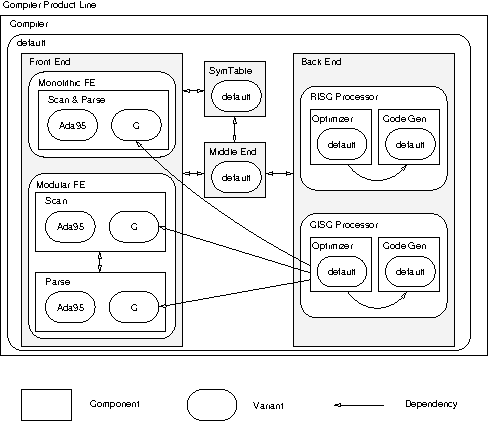
\includegraphics[width=15cm]{compiler-spl}
   \caption{Sicht des Produktlinieningenieurs}
\end{figure}
\subsection{Ansicht der Rolle eines Produktingenieurs}
\begin{figure}[ht]
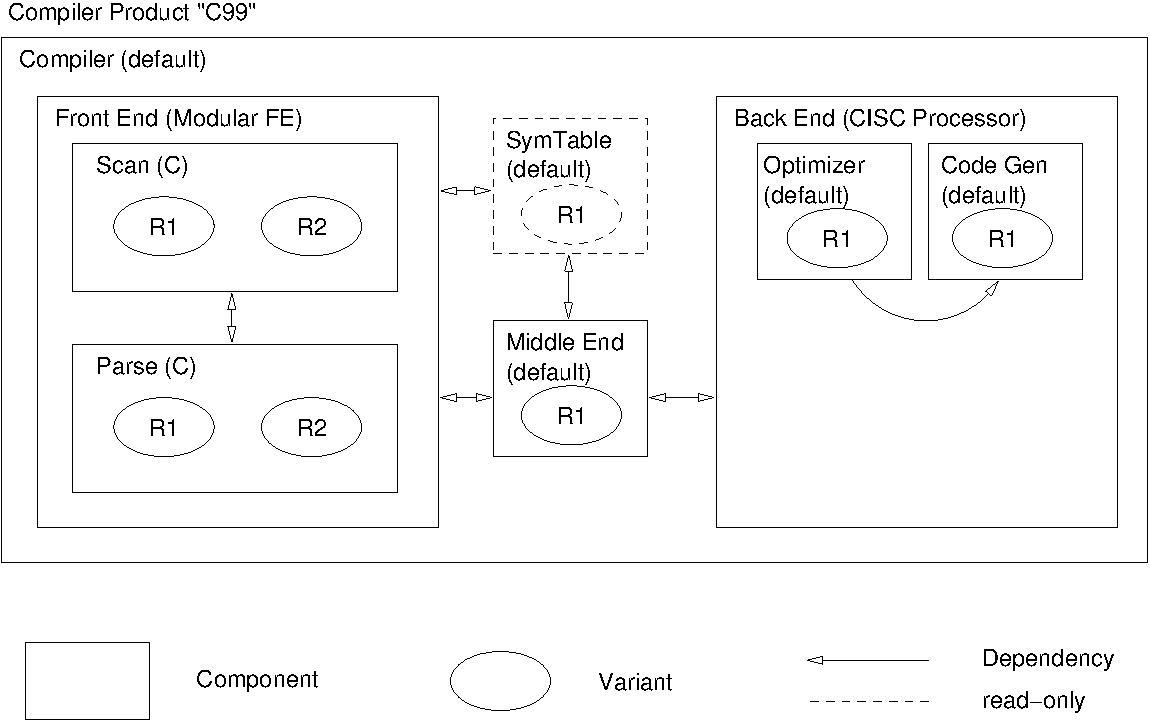
\includegraphics[width=15cm]{compiler-pe}
   \caption{Sicht des Produktingenieurs}
\end{figure}
\subsection{Ansicht der Rolle eines Programmierers}
\begin{figure}[ht]
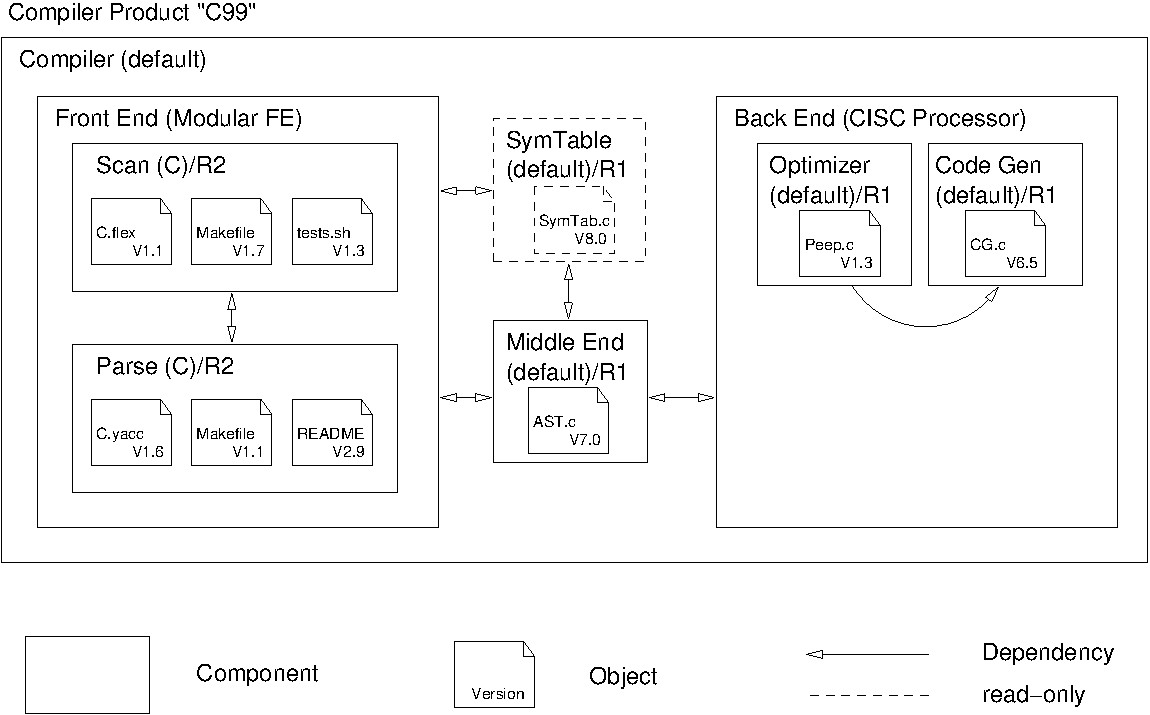
\includegraphics[width=15cm]{compiler-p}
   \caption{Sicht des Programmierers}
\end{figure}

\section{Der Rollen View}
Auf der linken Seite der Ausgangsperspektive wird ein hierarchischer Baum angezeigt, der
die momentan aktive Rolle und die mit Ihr verbundenen m�glichen Sichten darstellt.
\section{Der Worklflow/Task View}
Am unteren Rand der Ausgangsperspektive wird standardm�ssig 
\section{Die Minimap}
Am rechten unteren Rand der Ausgangsperspektive wird eine sogennante Minimap angezeigt,
in der ein �berblick �ber die ganze Architektursicht der aktuellen Rolle gegeben wird.

\section{Drools}

Kobold bietet seinem Benutzer einen Workflow-Mechanismus, der die Wahrung des definierten produktlinien-basierten 
Entwicklungsprozesses unterst�tzt. Dieser f�hrt Konsistenzpr�fungen durch, die in anderen Client-Instanzen 
automatisch Workflows  ansto�en, um die Inkonsistenz zu beheben.
Zur Realisierung des Workflow-Mechanismus wird die Rule Engine Drools\footnote{http://www.drools.org} 
verwendet.\par
Daf�r wird eine Regelbasis in XML f�r drool erzeugt. Diese besteht aus einer Menge aller Regelmengen und 
befindet sich auf dem Server. Eine Regelmenge wiederum besteht aus Regeln. Eine solche Regel gliedert 
sich in drei Teile: Parameter, Bedingung und Konsequenz. Dabei bilden die Parameter eventuell ben�tigte 
Parameter f�r die Regel. Die Bedingung �berpr�ft, ob die Regel angewendet wird oder nicht. Die Konsequenz
beeinhaltet die Aktionen, die durchgef�hrt werden, falls die Bedingung erf�llt ist.\par

Der Workflow-Mechanismus spielt sich sowohl auf dem Kobold Server als auch auf dem Kobold Client ab.\par

\subsection{Aktionen auf dem Kobold Server}
F�hrt ein Client eine Aktion aus, so wird diese dem Kobold Server gemeldet. Dieser wendet die Aktion als Fakt
auf die Regelbasis an, die sich auf dem Server befindet. Es werden dabei alle Regeln durchlaufen. Stimmt das 
Ereignis mit der Bedingung einer Regel �berein, so 
wird die Konsequenz dieser ausgef�hrt. Die Ergebnisse dieser Regelkonsequenzen werden zu einem 
Workflow-Objekt zusammengef�gt (zum Beispiel eine Reihe von Anweisungen). Ein Workflow-Objekt ist dabei 
eine Art XML-Struktur, die einen Titel und eine Liste aller Regelresultate 
besitzt. Diese Workflow-Objekt wird 
dann auf die Message-Queues der Clients gelegt, f�r die das Workflow-Objekt relevant ist. 

\subsection{Aktionen auf dem Kobold Client}
Sobald der Client eine Aktion ausf�hrt, meldet er diese dem Kobold Server um m�gliche Inkonsistenzen zu 
vermeiden. Wird ein Workflow entwickelt, so bekommt jeder Kobold Client, der den Workflow ansto�en sollte,
beim n�chsten Login dieses Objekt gepollt. Der Anwender wird dar�ber in der Workflow-View des Kobold Clients
informiert.\newline
\newline
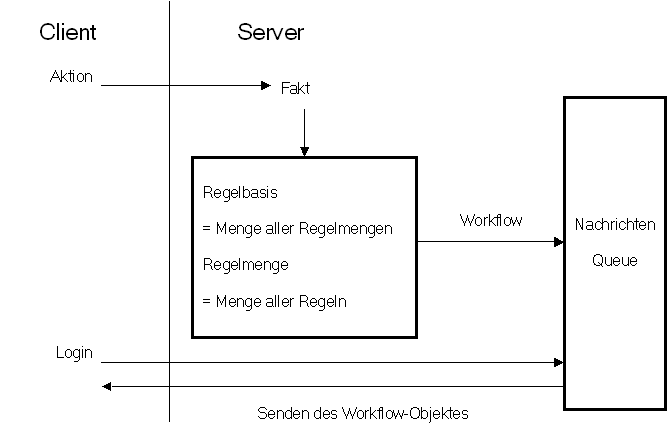
\includegraphics[width=15cm]{drools.png}\newline

\subsection{Die Regelbasis in Kobold}
Kobold wird in dieser Iteration eine Anfangsregelbasis zur Verf�gung stellen, die vom Anwender jederzeit erweitert werden 
kann. Er muss dabei eine neue Regel erstellen und sie der Regelbasis hinzuf�gen. Diese Regeln m�ssen dann 
nicht unbedingt zum 
Workflow-Objekt hinzugef�gt werden, sondern k�nnen in ihrer Konsequenz auch andere Aktionen ausf�hren. 
Dies bleibt dem Anwender �berlassen. Zur Erstellung einer neuen Regel wird ihm au�erdem ein Editor 
zur Verf�gung stehen, 
der in einer der kommenden Iterationen entstehen wird. 
\subsubsection{GXL Import und Export Funktionalit�t}
Da bei der Erstellung dieses Dokumentes noch kein �bereinkommen mit 
dem Auftraggeber getroffen werden konnte, und dieses auch erst in den n�chsten
Wochen m�glich sein wird, wird in diesem Fall nur eine sehr grobe Spezifikation 
vorgenommen. Grunds�tzlich ist vorgesehen, dass der GXL Import / Export in 
einem separaten Plugin realisiert wird, das zum Feature-Set geh�rt. 
Es ist vorgesehen, sowohl die Daten des Architekturgraphen, als auch die 
Daten, die auf Dateiebene hinter der Darstellung stehen, exportieren zu k�nnen. 
So werden bei einem Export die Architektur-Daten in Form einer XML Datei, 
die dem mit dem Kunden noch zu spezifizierenden GXL Schema entspricht, gespeichert.
Die mit der Architektur zusammenh�ngenden Assets werden in einem .jar File 
exportiert. Dies schlie�t Meta Informationen aus.
\chapter{Produktanatomie}

\section{Leistungsanforderungen}
Das System wird zun?chst so ausgelegt, dass mind. 50 Benutzer gleichzeitig mit dem Produkt arbeiten k?nnen.
Die Skalierbarkeit h?ngt ausschliesslich von dem Server ab, dessen Leistungsf?higkeit von der Hardware und
der verwendeten Persistenzschicht-Implementierung beeinflusst wird. Garantiert wird die Bereitstellung von 
10 Produktlinien zu je 50 Produkten. Pro Produktlinie k?nnen 100 Benutzer verwaltet werden.

\section{Minimale Hardwareanforderungen}
Das Softwaresystem wird auf einem Pentium II basierten PC mit 400 Mhz CPU-Takt, 256 MB Hauptspeicher
und mind. 200 MB freien Festplattenspeicher (oder unter einer vergleichbaren Unix-Workstation)
unter den Betriebssystemen Windows, Solaris und Linux lauff?hig sein.

\section{Entwurfseinschr?nkungen}
Das Produkt wird in Java 2 Version 1.4.1.3 implementiert. Als Workbench-Framework wird die 
Eclipse Plattform\footnote{http://www.eclipse.org/, http://www.eclipse.org/platform/}
verwendet, sowie deren Widgettoolkit SWT\footnote{Standard Widget Toolkit, http://www.eclipse.org/swt/}
und GEF\footnote{Graphical Editing Framework, http://www.eclipse.org/gef/}.
Zudem werden Bibliotheken von der Apache Software
Foundation\footnote{http://www.apache.org/} benutzt. Die
Generierung der Dokumenation setzt auf iText\footnote{http://www.lowagie.com/iText/} auf.

\section{Verf?gbarkeit}
F?r den Client gibt es keine besonderen Anforderungen bzgl. der Verf?gbarkeit. Die Verf?gbarkeit des Servers
h?ngt ma?geblich von der Konfiguration des Rechners ab, der den Serverdienst zur Vef?gung stellt.

\section{Sicherheit}
Die Daten, die der Server bereitstellt, werden bei jeder ?nderung sofort auf dem Datentr?ger gespeichert.
Somit wird die Gefahr eines Datenverlusts beim Eintritt von unvorhersehbaren Ereignissen minimiert.
Alle Client-spezifischen Daten werden in den Produktlinien- bzw.
Produkt-Repositories gespeichert und unterliegen  den Sicherheitsregeln des verwendeten
Versionskontrollsystems.

\section{Robustheit}
Fehleingaben und Fehler im System werden erkannt und dem Benutzer mit einer aussagekr?ftigen 
Fehlermeldung mitgeteilt.
Sie f?hren nicht zum Programmabsturz.

\section{Wartbarkeit}
Durch die st?ndige ?berpr?fung des Programmquellcodes mit Metriken auf Kopplung, Zusammenhalt und
Styleguide-Konformit?t wird die hohe Wartbarkeit des 
Produkts gew?hrleistet. Zudem wird das Produkt mit einer umfangreichen
Regression-Testsuite f?r die Nicht-GUI-Komponenten ausgeliefert.

\section{Performance}
%Das Softwaresystem soll laut Kundenangaben auf einem handels?blichen
%Pentium II PC mit mind. 400 Mhz CPU-Takt, mind. 256 MB Hauptspeicher
%und 200 MB freien Festplattenspeicher (oder auf einer vergleichbare Unix-Workstation)
%unter den Betriebssystemen Windows, Solaris oder Linux lauff?hig sein.
%Das System soll es erm?glichen die Produkt(-linien) Architekturen als Graph zu
%visualisieren.
%Es wurde nicht gefordert den ganzen Graphen, der unter Umst?nden sehr komplex und 
%gro? werden kann, auf einmal performant zu visualisieren.\par
%Es gen?gt die f?r die 
%jeweilige Architekturansicht relevanten Teile des Graphen zu visualisieren.
%Diese Ausschnitte werden sich der ?bersichtlichkeit halber wahrscheinlich in einer 
%Gr??enordnung bis zu 125 Knoten bewegen. Die Anzeige der Teilgraphen sollte 
%eine Grenze von 8 Sekunden zur Berechnung der Darstellung nicht ?berschreiten.
Es wurde nicht gefordert den ganzen Graphen, der unter Umst?nden sehr komplex
werden kann, performant zu visualisieren.\par
Es soll gen?gen, die f?r die jeweilige Architekturansicht relevanten
Ausschnitte des Graphen zu visualisieren.
Diese werden sich der ?bersichtlichkeit proforma in einer 
Gr??enordnung bis zu 125 Knoten bewegen. Die Anzeige der Teilgraphen sollte 
eine Grenze von 8 Sekunden zur Berechnung der Darstellung nicht ?berschreiten.

\section{Portabilit?t}
Der Server st?tzt sich auf keine nativen Schnittstellen sondern benutzt ausschlie?lich 
\emph{pure java}. Somit ist er laut Sun Microsystems 
Inc.\footnote{unter http://java.sun.com/j2se/1.4.2/system-configurations.html} unter 
Solaris-SPARC, Solaris-Intel, Windows NT/2000/XP und Linux lauff?hig.


\chapter{Server}
Der Server wird als HTTP-basierter {\it XML-RPC Server}
\footnote{N?here Informationen: http://ws.apache.org/xmlrpc/}
implementiert und ist SSL-basiert. Ausserdem erm?glicht
der Server eine Client-zu-Client-Kommunikation ?ber eine Nachrichten-Queue, welche
in regelm?ssigen Abst?nden von den Clients abgefragt wird (Request/Response).
Alle Informationen, die der Server bereitstellt sind persistent.\par
Die Wartung des Servers wird durch ein kommandozeilen-orientiertes
Administrationstool realisiert.\newline

F?r jeden Benutzer werden folgende Daten gespeichert:
\begin{itemize}
\item Benutzername
\item Passwort
\item eMail
\item Name
\item Liste von Rollen
\end{itemize}

Eine Rolle besteht aus einer Liste von Produkten und Produktlinien.\newline
F?r jedes Element in der Liste wird au?erdem noch eine Liste der zugeh?rigen Repositories angeh?ngt. 
Ist das Element ein Produkt, so werden auch die Daten der dazugeh?rigen Produktlinie erfasst.\newline

F?r ein Repository werden folgende Daten gespeichert:
\begin{itemize}
\item Pfad
\item Passwort
\item Benutzername
\item Schreibrecht (ja/nein)
\end{itemize}

\section{Berechtigungskonzept}

Zur Realisierung des produktlinien\-?bergreifenden Berechtigungskonzepts
verwaltet der Server alle benutzer-, rollen-, produktlinien- und
produkt-basierten Berechtigungen. Dabei kann ein Server produktlinien-?bergreifend
verwendet werden.\par
Der Server bietet ein auf diesen Berechtigungen basierenden
Authentifizierungsmechanismus an, der von allen Clients verwendet wird.

\section{Persistierung}

Die Persistierung aller f?r das Berechtigungskonzept notwendigen Daten wird
durch eine abstrakte Persistenzschicht realisiert, die es erm?glicht, die
Datenhaltung flexibel zu organisieren. Im Rahmen dieses Angebotes wird die
Persistierung XML-basiert angeboten.

\section{Nachrichten-Queue}

Die vom Server angebotene Nachrichten-Queue ist zustandsbehaftet, d.h. nach einem
Stromausfall oder anderen unvorhersehbaren Ereignissen ist die Nachrichten-Queue
in der Regel ohne Datenverlust wiederherstellbar.\par
Dadurch wird ein hoher Grad an Konsistenztreue und Zuverl?ssigkeit erreicht.\newline

F?r die Nachrichten-Queue werden folgende Daten ben?tigt:
\begin{itemize}
\item von wem
\item an wen
\item Inhalt
\item Datum
\item ID
\item Priorit?t
\end{itemize}



\section{Web-basierte Statusinformationen}

Es ist jederzeit f?r einen authentifizierten Systemadministrator m?glich,
den Status des Servers ?ber einen Webbrowser abzufragen.

\section{Administrationstool}

Zur Administration des Servers wird ein kommandozeilen-orientiertes 
Administrationstool angeboten, dass es erm?glicht, Produktlinien-Ingenieur-Accounts
anzulegen bzw. zu entfernen, die Nachrichten-Queue zu
leeren und den Server zu starten oder zu stoppen.


\section{Metainformationskomponente}

F?r die Elemente in Kobold werden unterschiedliche Metainformationen gespeichert. Dieses Kapitel liefert eine genaue Auflistung der geplanten Metadaten.\newline

\textbf{Produkt:}\par
Das Produkt wird vom Produktingenieur bearbeitet und entsteht aus der Architektur der Produktlinie. 
\begin{itemize}
\item letztes Release\newline
\end{itemize}

\textbf{Release:}\par
Ein Release besteht aus einer Gruppe von Objekten (Source Code, Dokumentation, etc.) in einem Zustand, in dem sie als Teil des fertigen Produktes eingesetzt werden kann.
\begin{itemize}
\item Liste der Dateien (mit Versionsangabe)
\item Liste der zus?tzlichen Objekte
\item Liste der Skripte
\item Erstellungsdatum\newline
\end{itemize}

\textbf{Version:}\par
Objekte (Source Code, Dokumentation, etc.) sind in unterschiedlichen Versionen verf?gbar. Die Versionskontrolle ?bernimmt dabei eine Standard Versiosverwaltungssystem wie zum Beispiel CVS, RCS, etc.
\begin{itemize}
\item Liste der Skripte
\item Status\newline
\end{itemize}

\textbf{Datei:}\par
Eine Datei ist ein Objekt, das Source Code enth?lt.
\begin{itemize}
\item Liste der Versionen
\item ID
\item Name
\item bin?r (ja/nein)
\item Beschreibung\newline
\end{itemize}

\textbf{Variante:}\par
Eine Variante besteht entweder aus weiteren Komponenten oder aus Releases.
\begin{itemize}
\item Liste aller Dateien
\item Versionsnummer
\item Zust?ndiger
\item Name
\item Beschreibung
\item ID
\item Liste der Skripte
\item Status\newline
\end{itemize}

\textbf{Komponente:}\par
Eine Komponente besteht aus einer oder mehreren Varianten.
\begin{itemize}
\item Liste aller Varianten
\item Name
\item Zust?ndiger
\item Beschreibung
\item ID
\item Liste der Skripte
\item Status\newline
\end{itemize}

\textbf{Abh?ngigkeit:}\par
Eine Abh?ngigkeit besteht zwischen zwei Knoten der Architektur. F?r Abh?ngigkeiten zwischen mehr als zwei Knoten werden Metaknoten verwendet.
\begin{itemize}
\item Typ
\item Richtung
\item Knoten1
\item Knoten2
\item weiter beliebig attributierbar\newline
\end{itemize}

\textbf{Metaknoten:}\par
Metaknoten werden f?r Mehrfachbeziehungen verwendet.
\begin{itemize}
\item Typ
\item ID\newline
\end{itemize}

\textbf{Architektur:}\par
Eine Architektur stellt sowohl ein Produkt als auch eine Produktlinie graphisch dar.
\begin{itemize}
\item Liste der Metaknoten
\item Liste der Abh?ngigkeiten
\item Liste der Komponenten (oberste Ebene)
\item Name
\item Typ
\item Status
\item Zust?ndiger
\item Link auf das Repository
\item Liste der Skripte
\end{itemize}


\section{Repository Abstraction Layer:}

Zur besseren Kommunikation mit der Server, soll ein Repository Abstraction Layer erstellt werden, das mit der Authentifizierung am Server umgehen kann. Dieses vermittelt zwischen Kobold und dem VCM der Eclipse-Komponente.\newline

Das Repository Abstraction Layer behandelt Anfragen an den Server, indem es diese entweder an das eigentliche VCM weiterleitet, oder mit einer passenden Meldung ablehnt.\par
Ist in der Eclipse-Komponente noch nicht der Pfad eines Repositories gespeichert, so holt sich das Repository Abstraction Layer die n?tigen Informationen vom Server und speichert diese in der Eclipse-Komponente.



\chapter{Server}

Dieser Abschnitt beschreibt die Komponenten des Entwurfs des
Kobold Servers. In der Iteratrion 1 untergliedert sich der Server
in 5 Komponenten. Man beachte insbesondere auch das Kapitel 2.3
der Spezifikation1, das die Anforderungen an die jeweiligen
Komponenten spezifiziert.

\section{�berblick}
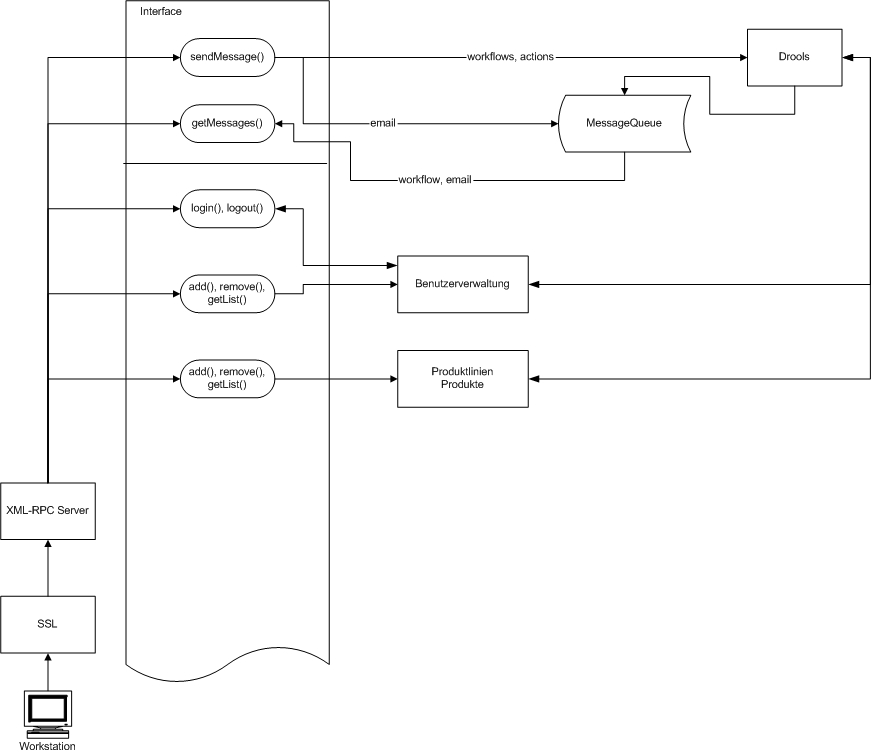
\includegraphics[width=15cm]{server.jpg}

\section{Komponente Kobold Interface}

Die Komponente Interface bildet die Schnittstelle des Kobold
Servers nach aussen und ist dessen Einsprungklasse. Sie wird von
den Kobold Clients �ber remote procedure calls angesprochen.
Anfragen werden an die daf�r zust�ndigen Komponenten des Kobold
Servers delegiert.

\section{Komponente WorkflowEngine}

Diese Komponente erh�lt Daten �ber durchgef�hrte (VCM-)Actionen
sowie Workflowobjekte, die auf die vorhandenen Regelmengen
angewendet werden. Daf�r k�nnen ben�tigte Daten von den
Komponenten Benutzerverwaltung und Produktlinienverwaltung
abgerufen werden. Als Konsequenz k�nnen Workflows oder EMails an
die MessageQueue-Komponente �bergeben werden.

\section{Komponente MessageQueue}

Aufgabe dieser Komponente ist die Verwaltung und Zustellung von
Worklows und EMails an die addressierten Clients, sobald diese
getMessages() aufrufen.

\section{Komponente Benutzerverwaltung}

Die Benutzerverwaltung ist zust�ndig f�r die Authentifizierung der
Benutzer beim Login und verwaltet deren Rollendaten. S�mtliche
Benutzerdaten k�nnen von dieser Komponente abgefragt werden.

\section{Komponente Produktlinien-/Produktverwaltung}

Diese Komponente verwaltet s�mtliche auf dem Server zu
persistierende Daten zu Produktlinien und Produkten.

\chapter{Nichtfunktionale Anforderungen}
\section{Leistungsanforderungen}
Das System wird zun�chst so ausgelegt, dass mind. 50 Benutzer gleichzeitig mit dem Produkt arbeiten k�nnen.
Die Skalierbarkeit h�ngt ausschliesslich vom Server ab, dessen Leistungsf�higkeit von der Hardware und
der verwendeten Persistenzschicht-Implementierung beeinflusst wird. Garantiert wird die Bereitstellung von 
10 Produktlinien zu je 50 Produkten. Pro Produktlinie k�nnen 100 Benutzer verwaltet werden.

\section{Minimale Hardwareanforderungen}
Das Softwaresystem wird auf einem Pentium II basierten PC mit 400 Mhz CPU-Takt, 256 MB Hauptspeicher
und mind. 200 MB freien Festplattenspeicher (oder unter einer vergleichbaren Unix-Workstation)
unter den Betriebssystemen Windows, Solaris und Linux lauff�hig sein.

\section{Entwurfseinschr�nkungen}
Das Produkt wird in Java 2 Version 1.4 implementiert. Als Workbench-Framework wird die 
Eclipse Plattform\footnote{http://www.eclipse.org/, http://www.eclipse.org/platform/}
verwendet, sowie deren Widgettoolkit SWT\footnote{Standard Widget Toolkit, http://www.eclipse.org/swt/}
und GEF\footnote{Graphical Editing Framework, http://www.eclipse.org/gef/}.
Zudem werden Bibliotheken von der Apache Software
Foundation\footnote{http://www.apache.org/} benutzt. Die
Generierung der Dokumenation setzt auf iText\footnote{http://www.lowagie.com/iText/} auf.

\section{Verf�gbarkeit}
F�r den Client gibt es keine besonderen Anforderungen bzgl. der Verf�gbarkeit. Der Kobold-Serverdienst soll mit mind. 99\% hoch verf�gbar sein. 
Die Server-Verf�gbarkeit h�ngt trotzdem von der Konfiguration des Rechners, der den Serverdienst zur Verf�gung stellt, ab.

\section{Sicherheit}
Die Daten, die der Server bereitstellt, werden bei jeder �nderung sofort auf dem Datentr�ger gespeichert.
Somit wird die Gefahr eines Datenverlusts beim Eintritt von unvorhersehbaren Ereignissen minimiert.
Alle Client-spezifischen Daten werden in den Produktlinien- bzw.
Produkt-Repositories gespeichert und unterliegen  den Sicherheitsregeln des verwendeten
Versionskontrollsystems.

\section{Robustheit}
Fehleingaben und Fehler im System werden erkannt und dem Benutzer mit einer aussagekr�ftigen 
Fehlermeldung mitgeteilt. Sie f�hren nicht zum Programmabsturz. Genaueres folgt in einer sp�teren Iteration.

\section{Wartbarkeit}
Durch die st�ndige �berpr�fung des Programmquellcodes mit Metriken auf Kopplung, Zusammenhalt und
Styleguide-Konformit�t wird die hohe Wartbarkeit des 
Produkts gew�hrleistet.

\section{Performance}
%Das Softwaresystem soll laut Kundenangaben auf einem handels�blichen
%Pentium II PC mit mind. 400 Mhz CPU-Takt, mind. 256 MB Hauptspeicher
%und 200 MB freien Festplattenspeicher (oder auf einer vergleichbare Unix-Workstation)
%unter den Betriebssystemen Windows, Solaris oder Linux lauff�hig sein.
%Das System soll es erm�glichen die Produkt(-linien) Architekturen als Graph zu
%visualisieren.
%Es wurde nicht gefordert den ganzen Graphen, der unter Umst�nden sehr komplex und 
%gro� werden kann, auf einmal performant zu visualisieren.\par
%Es gen�gt die f�r die 
%jeweilige Architekturansicht relevanten Teile des Graphen zu visualisieren.
%Diese Ausschnitte werden sich der �bersichtlichkeit halber wahrscheinlich in einer 
%Gr��enordnung bis zu 125 Knoten bewegen. Die Anzeige der Teilgraphen sollte 
%eine Grenze von 8 Sekunden zur Berechnung der Darstellung nicht �berschreiten.
Es wurde nicht gefordert den ganzen Graphen, der unter Umst�nden sehr komplex
werden kann, performant zu visualisieren.\par
Es soll gen�gen, die f�r die jeweilige Architekturansicht relevanten
Ausschnitte des Graphen zu visualisieren.
Diese werden sich der �bersichtlichkeit proforma in einer 
Gr��enordnung bis zu 125 Knoten bewegen. Die Anzeige der Teilgraphen sollte 
eine Grenze von 8 Sekunden zur Berechnung der Darstellung nicht �berschreiten.

\section{Portabilit�t}
Der Server st�tzt sich auf keine nativen Schnittstellen sondern benutzt ausschlie�lich 
\emph{pure java}. Somit ist er laut Sun Microsystems 
Inc.\footnote{unter http://java.sun.com/j2se/1.4.2/system-configurations.html} unter 
Solaris-SPARC, Solaris-Intel, Windows NT/2000/XP und Linux lauff�hig.

Der Client basiert grundlegend auf der Eclipse Plattform und deren Widgettoolkit und ist
dadurch von dessen nativer Schnittstelle abh�ngig. Laut dem Eclipse Consortium werden die folgenden 
Plattformen und Betriebssysteme unterst�tzt:
\begin{itemize}
    \item Windows NT/2000/XP
    \item Linux (Motif)
    \item Linux (GTK 2)
    \item Solaris 8 (SPARC/Motif)
    \item QNX (x86/Photon)
    \item AIX (PPC/Motif) 
    \item HP-UX (HP9000/Motif)
    \item Mac OSX (Mac/Cocoa)
\end{itemize}





%%%%%%%%%%%%%%%%%%%%%%%%%%%%%%%%%%%%%%%%%%%%%%%%%%%%%%%%%%%%%%%%%%%%%%%%%%%%%%%
%% Anhang
\appendix
%%%%%%%%%%%%%%%%%%%%%%%%%%%%%%%%%%%%%%%%%%%%%%%%%%%%%%%%%%%%%%%%%%%%%%%%%%%%%%%
%% StuPro A, Produktlinien (Kobold)
%% Team Werkbold
%% Angebot
%% $Id: begriffslexikon.tex,v 1.6 2004/02/19 14:04:10 grosseml Exp $
%%%%%%%%%%%%%%%%%%%%%%%%%%%%%%%%%%%%%%%%%%%%%%%%%%%%%%%%%%%%%%%%%%%%%%%%%%%%%%%
\newcommand{\begriff}[2]
{\item \bfseries{#1} \textnormal{#2}}

\chapter{Begriffslexikon}
\begin{itemize}

\begriff{Ansicht}{Eine rollenabh�ngige Sicht}

\begriff{Arbeitskopie}{Kopie, mit der gearbeitet wird und die tats�chlich ver�ndert wird}

\begriff{Architektur}{Struktur von Software, die aus Komponenten und
Konnektoren besteht}

\begriff{Auschecken}{VCM-Funktion zum Anfordern einer Arbeitskopie aus dem Repository}

\begriff{Assets}{Wiederverwendbare Komponenten, z.B. Source-Pakete, Klassen,
usw.}

\begriff{Core-Assets}{Architekturkomponenten, die bestimmte Funktionalit�ten 
erf�llen und oft wiederverwendet werden. Sie bilden mit den produktspezifischen 
Komponenten das Produkt}

\begriff{Core-Asset-Entwickler}{Softwareentwickler, der Core-Assets entwickelt}

\begriff{Core-Asset-Repository}{Entwicklungs-Repository (Arbeitskopie) der
Core-Assets}

\begriff{Deprecated}{Veraltet, missbilligend}

\begriff{Einchecken}{VCM-Funktion zum R�ckschreiben der Arbeitskopie-�nderungen
ins Repository}

\begriff{Entwicklungs Repository} {Siehe Arbeitskopie}

\begriff{Erstentwicklung}{Entwicklung eines neuen Produkts bzw. eines neuen 
Core-Assets}

\begriff{Evolution�res Vorgehensmodell}{Inkrementelles Vorgehensmodell in der
Softwareentwicklung, �hnlich dem Spiralmodell nach B.W. Boehm}

\begriff{Fakt}{eine Mitteilung an den Kobold-Server}

\begriff{Feature-Set}{Ein Plugin-Satz zur Erweiterung von Eclipse, so dass 
Eclipse nach der Erweiterung ein eigenes Erscheinungsbild hat}

\begriff{Iteration}{Phase im evolution�ren Vorgehensmodell}

\begriff{Kernkomponenten}{siehe Core-Assets}

\begriff{Komponenten}{Bestandteile der Produktlinien- bzw. Produktarchitektur}

\begriff{Message-Queue}{Nachrichten, die auf Anfrage an den Benutzer geleitet werden}

\begriff{Metainformation}{Zusatz-Informationen �ber Informationen}

\begriff{Module}{siehe Komponenten}

\begriff{Plugin}{Softwarekomponente, die die Funktionalit�t des Systems erweitert}

\begriff{Produktarchitektur}{Software-Architektur eines Produktes}

\begriff{Produkt-Entwickler}{P, Softwareentwickler dessen Vorgesetzter ein
Produkt-Ingenieur ist}

\begriff{Produkt-Ingenieur}{PE, ein Software-Ingenieur mit Leitungs- und 
Entscheidungskompetenz bzgl. der technischen Realisierung des Produkts. 
Der PE hat den Produktlinien-Ingenieur als Vorgesetzten.}

\begriff{Produktlinien-Ingenieur}{PLE, Software-Ingenieur mit projekt�bergreifender 
Leitungs- und Entscheidungskompetenz bzgl. der technischen Realisierung 
und Pflege der Produktlinienarchitektur.}

\begriff{Produkt-Repository}{Repository, das vom PE verwaltet wird, Entwickler
checken Arbeitskopien von Produkt�Komponenten aus}

\begriff{Produktlinien-Repository}{Repository, das vom PLE verwaltet wird, PE checken
Arbeitskopien von Core-Asset Varianten aus}

\begriff{Prototyp}{Entwicklungsversion eines Programmes}

\begriff{RPC}{Remote Procedure Call erlaubt die Ausf�hrung von Funktionen, 
die auf einem anderen Rechner implementiert sind}

\begriff{Repository}{Datei-Verwaltung zur Verwaltung von Versionen}

\begriff{Softwarearchitektur}{siehe Architektur}

\begriff{Update}{VCM-Funktion, die die Arbeitskopie mit dem Repository
synchronisiert}

\begriff{Varianten}{Modifikationen von Core-Assets}

\begriff{VCM}{Version Control Management, ein Versionsverwaltungssystem wie z.B.
das Versionsverwaltungstool CVS (Concurrent Versions System)}

\begriff{Version}{Eindeutige Bezeichnung zu einem fixen Zeitpunkt}

\begriff{View}{Subfenster von Kobold-Client}

\begriff{Wasserfall-Vorgehensmodell}{Klassisches Vorgehensmodell in der
Softwareentwicklung, das in Phasen aufgeteilt ist, die aufeinander folgen}

\begriff{Workflow}{Arbeits- bzw. Gesch�ftsprozess}

\end{itemize}

%%% Local Variables: 
%%% TeX-master: "angebot"
%%% End: 
%%% vim:tw=79:


\begin{thebibliography}{99}
	\bibitem {paper} Daniel Simon, Thomas Eisenbarth, Stefan Bellon, Gunther Vogel, J�rg Czeranski {\it PLAM - A Product Line Asset Management Tool}
\end{thebibliography}

\end{document}
%%% vim:tw=79:
